\section{Software State Machines}

\subsection{Introduction - FSM in Hardware vs Software}

\begin{definition}{Finite State Machine (FSM)}
A machine with a finite number of states and transitions, which responds to inputs based on its current state. It represents a computational model used to design both computer programs and sequential logic circuits. FSMs are particularly useful in embedded systems for controlling the behavior of the system in response to external events.
\end{definition}

\begin{concept}{Hardware vs Software FSM Implementation}
\paragraph{Hardware FSM}
\begin{itemize}
    \item Intrinsically parallel - multiple FSMs process simultaneously
    \item Clock-driven - inputs evaluated at clock edges
    \item Unchanged input signals create no overhead
    \item Uses flip-flops to store internal state
    \item State can only change on a clock edge
    \item Typically implemented as either Moore or Mealy machines
\end{itemize}

\paragraph{Software FSM}
\begin{itemize}
    \item Intrinsically sequential - CPU processes one FSM after another
    \item Event-driven - only evaluate FSM when inputs change
    \item Evaluating all inputs on each function call would waste CPU time
    \item Synchronization issues in sequential systems if using "synchronous clock approach"
    \item More flexibility in implementation patterns
    \item Better suited for complex state transitions and conditions
\end{itemize}
\end{concept}

\begin{example2}{Moore vs Mealy Hardware FSM}

// Moore FSM - Output depends only on state
Moore FSM:
\begin{itemize}
    \item State A (output: 0) $\rightarrow$ State B (output: 0)  // event: I=0
    \item State B (output: 0) $\rightarrow$ State C (output: 1)  // event: I=0
    \item State C (output: 1) $\rightarrow$ State D (output: 0)  // event: I=1
    \item State D (output: 0) $\rightarrow$ State A (output: 0)  // event: I=1
\end{itemize}

// Mealy FSM - Output depends on state and input
Mealy FSM:
\begin{itemize}
    \item State A (output: 0) $\rightarrow$ State B (output: 0)  // event: I=1
    \item State B (output: 1) $\rightarrow$ State A (output: 1)  // event: I=0
    \item State B (output: 0) $\rightarrow$ State C (output: 0)  // event: I=1
    \item State C (output: 1) $\rightarrow$ State A (output: 1)  // event: I=0
\end{itemize}
\end{example2}

\begin{definition}{Moore vs Mealy FSMs}
\paragraph{Moore FSM}
In a Moore FSM, the outputs are determined solely by the current state, not directly by the inputs.
\begin{center}
State $\rightarrow$ Output
\end{center}

\paragraph{Mealy FSM}
In a Mealy FSM, the outputs are determined by both the current state and the current inputs.
\begin{center}
(State, Input) $\rightarrow$ Output
\end{center}
\end{definition}

\subsection{Reactive Systems}

\begin{definition}{Reactive System (State-Event Model)}
A system that responds to external events (inputs) based on its internal state. It is event-driven and processes events as they occur, rather than evaluating all inputs periodically. Reactive systems are particularly well-suited for implementing FSMs in software because they minimize CPU overhead.
\end{definition}

\begin{concept}{Components of a Reactive System}
\begin{itemize}
    \item \textbf{Events:} External inputs that trigger the system's response
    \item \textbf{Internal state:} Memory of what happened before
    \item \textbf{Actions:} Influence on the outside world (outputs)
    \item \textbf{Transitions:} Rules for how events change state and trigger actions
\end{itemize}

The key advantage of the reactive approach is that the FSM is evaluated only when an input changes, reducing processing overhead compared to polling all inputs regularly.
\end{concept}

\begin{example}
Common applications of state-event models include:
\begin{itemize}
    \item Communication protocols (connection establishment, data transfer, connection termination)
    \item Human-machine interfaces (input recognition and validation)
    \item Parsing of programming languages and text
    \item Process control systems (washing machines, vending machines, heating systems)
    \item Embedded control systems (automotive, medical devices)
\end{itemize}
\end{example}

\subsection{Modeling State Machines in UML}

\begin{definition}{UML State Diagram}
A graphical representation based on the Unified Modeling Language (UML) for modeling finite state machines. Based on the notation developed by Prof. David Harel, it describes the reactive behavior of systems. UML state diagrams provide a standard way to document and communicate the behavior of state-based systems.
\end{definition}

\begin{concept}{UML State Diagram Elements}
\begin{itemize}
    \item \textbf{State:} Internal condition of the system waiting for the next event
    \item \textbf{Event:} Asynchronous input that may cause a transition
    \item \textbf{Transition:} Reaction to an event, may change state and/or trigger an action
    \item \textbf{Action:} Output associated with a transition (written after a forward slash)
    \item \textbf{Initial state:} Default starting state of the system (indicated by a solid circle)
    \item \textbf{Default transition:} Arrow from initial state to the first active state
\end{itemize}

In contrast to hardware FSM notations like Mealy, UML state diagrams:
\begin{itemize}
    \item Treat inputs as asynchronous events rather than signal levels
    \item Treat outputs as actions
    \item Omit inputs that have no effect (increasing diagram clarity)
    \item Can represent both Mealy and Moore behaviors in a unified notation
\end{itemize}
\end{concept}

\begin{example}
Simple light switch state diagram in UML:

\begin{center}
state\_off $\rightarrow$ state\_on (event: on / action: lamp\_on)\\
state\_on $\rightarrow$ state\_off (event: off / action: lamp\_off)
\end{center}

With an initial default transition to state\_off.

Note that the transition "off" in state\_off is not shown because it would have no effect and trigger no action.
\end{example}

\begin{examplecode}{Traffic Light Controller}
// UML state diagram for a simple traffic light controller

Initial state $\rightarrow$ Red

Red $\rightarrow$ Red\_Yellow (event: timer\_expired / action: set\_red\_yellow)
Red\_Yellow $\rightarrow$ Green (event: timer\_expired / action: set\_green)
Green $\rightarrow$ Yellow (event: timer\_expired / action: set\_yellow) 
Yellow $\rightarrow$ Red (event: timer\_expired / action: set\_red)

// Each state has an associated timer that generates 
// a timer\_expired event after a state-specific duration
\end{examplecode}

\begin{KR}{UML State Diagram Design Rules}
\paragraph{Basic Rules}
\begin{itemize}
    \item Every state diagram must have an initial state
    \item Each state has to be reachable through a transition
    \item The state diagram has to be deterministic - for each event it has to be defined which transition is triggered
    \item Avoid inconsistent or contradictory transitions that could lead to ambiguity
\end{itemize}

\paragraph{Semantics of UML FSM}
\begin{itemize}
    \item FSM is passive - only reacts to events from outside
    \item Always has a defined state
    \item Reaction depends on current state
    \item Event is discarded if no transition exists for it in current state
    \item Run-to-completion - once started, a transition cannot be interrupted
    \item Strives to avoid querying additional input - transitions should depend only on the event, not additional inputs
\end{itemize}
\end{KR}

\begin{example2}{Motor Control FSM Example}
Consider a motor control system with the following requirements:
\begin{itemize}
    \item Operator can turn motor on/off using start/stop buttons
    \item System shuts down motor if temperature limit is exceeded
    \item Restarting after temperature shutdown requires acknowledging the fault
    \item Normal operation and alarm conditions have different indicator lamps
\end{itemize}

UML state diagram would include:
\begin{itemize}
    \item States: idle, operate, fault, wait\_ack
    \item Events: start, stop, ack, t\_limit\_exceeded, t\_normalized
    \item Actions: motor\_on, motor\_off, op\_lamp\_on, op\_lamp\_off, al\_lamp\_on, al\_lamp\_off
\end{itemize}

Key transitions:
\begin{itemize}
    \item idle $\rightarrow$ operate (event: start / action: motor\_on, op\_lamp\_on)
    \item operate $\rightarrow$ idle (event: stop / action: motor\_off, op\_lamp\_off)
    \item operate $\rightarrow$ fault (event: t\_limit\_exceeded / action: motor\_off, op\_lamp\_off, al\_lamp\_on)
    \item fault $\rightarrow$ wait\_ack (event: t\_normalized / action: al\_lamp\_off)
    \item wait\_ack $\rightarrow$ idle (event: ack)
\end{itemize}
\end{example2}

\subsection{Implementation in C}

\begin{concept}{Basic Implementation Structure}
Software implementation of a state machine typically uses two main functions:
\begin{itemize}
    \item \textbf{fsm\_init():} Initializes the state machine to its default state
    \item \textbf{fsm\_handle\_event(event):} Processes an incoming event based on current state
\end{itemize}

The main program continuously polls for events and passes them to the state machine when they occur. This separation of event detection and processing is key to the efficiency of software FSMs.
\end{concept}

\begin{code}{FSM Implementation Pattern}
\begin{lstlisting}[language=C, style=basesmol]
// State and event enumerations
typedef enum {
    STATE_A,
    STATE_B,
    STATE_C,
    // ...other states
} state_t;

typedef enum {
    NO_EVENT,
    EVENT_X,
    EVENT_Y,
    // ...other events
} event_t;

// Current state variable
static state_t state;

// Initialization function
void fsm_init(void) {
    state = STATE_A;  // Set initial state
    // Additional initialization if needed
}

// Event handler function
void fsm_handle_event(event_t event) {
    switch (state) {
        case STATE_A:
            switch (event) {
                case EVENT_X:
                    action1();
                    state = STATE_B;
                    break;
                case EVENT_Y:
                    action2();
                    // No state change
                    break;
                default:
                    // Event ignored in this state
                    break;
            }
            break;
        case STATE_B:
            // Handle events for state B
            break;
        // Other states
    }
}

// Main loop
int main(void) {
    event_t event;
    
    fsm_init();
    
    while (1) {
        event = get_event();
        if (event != NO_EVENT) {
            fsm_handle_event(event);
        }
    }
}
\end{lstlisting}
\end{code}

\begin{examplecode}{LED Control FSM Implementation}
\begin{lstlisting}[language=C, style=basesmol]
// State and event definitions
typedef enum {
    STATE_OFF,
    STATE_ON
} state_t;

typedef enum {
    NO_SWITCH,
    S0,
    S1
} event_t;

// Current state
static state_t state = STATE_OFF;

// Initialize the FSM
void fsm_init(void) {
    state = STATE_OFF;
    // Initialize hardware, ensure LED is off
    led_off();
}

// Handle incoming events
void fsm_handle_event(event_t event) {
    switch (state) {
        case STATE_OFF:
            if (event == S0) {
                led_on();  // Action
                state = STATE_ON;  // State transition
            }
            break;
        case STATE_ON:
            if (event == S0) {
                led_off();  // Action
                state = STATE_OFF;  // State transition
            }
            break;
    }
}

// Event detection function
event_t get_event(void) {
    // Read hardware inputs
    uint32_t switches = read_switches();
    
    // Check switch positions
    if (switch_changed(switches, 0)) {
        return S0;
    } else if (switch_changed(switches, 1)) {
        return S1;
    }
    
    return NO_SWITCH;  // No event
}

// Main program
int main(void) {
    event_t event;
    
    // System initialization
    peripherals_init();
    fsm_init();
    
    // Main loop
    while (1) {
        event = get_event();
        if (event != NO_SWITCH) {
            fsm_handle_event(event);
        }
    }
}
\end{lstlisting}
\end{examplecode}

\subsection{Interaction of FSMs}

\begin{definition}{FSM Interaction Components}
\begin{itemize}
    \item \textbf{Port:} Defines the messages that can be sent and received by an FSM
        \begin{itemize}
            \item Output message $\rightarrow$ action of the FSM
            \item Input message $\rightarrow$ event for the FSM
        \end{itemize}
    \item \textbf{Link:} Defines a connection for sending messages between FSMs
    \item \textbf{Event Queue:} Buffer for events generated by different objects
\end{itemize}
\end{definition}

\begin{concept}{Event Queue for FSM Interaction}
\begin{itemize}
    \item Collects events generated by different objects
    \item Buffered to avoid losing events (especially important in interrupt-driven systems)
    \item FSM processes one event after the other
    \item Events are deleted after processing
    \item Provides decoupling between event producers and consumers
\end{itemize}

Actions of one FSM become events for another FSM, allowing complex systems to be constructed from simpler components. This approach enables modular design and clear separation of concerns.
\end{concept}

\begin{example}
A lamp FSM reacts to events created by a button FSM:

Button FSM states: released, pressed\\
Button port: out (pressed, released)

Lamp FSM states: off, on\\
Lamp port: in (pressed, released)

Button transitions:
\begin{itemize}
    \item released $\rightarrow$ pressed / out.pressed
    \item pressed $\rightarrow$ released / out.released
\end{itemize}

Lamp transitions:
\begin{itemize}
    \item off $\rightarrow$ on (on event in.pressed)
    \item on $\rightarrow$ off (on event in.released)
\end{itemize}

The communication between these two FSMs happens through messages passed via their ports.
\end{example}

\begin{KR}{Building Event-Based FSM Systems}
\paragraph{System Structure}
\begin{itemize}
    \item Divide system into multiple FSMs with well-defined responsibilities
    \item Define ports and interfaces for each FSM
    \item Connect FSMs through links and event queues
    \item Keep individual FSMs simple and focused on specific tasks
\end{itemize}

\paragraph{Implementation}
\begin{itemize}
    \item Use interrupt service routines (ISRs) to capture hardware events
    \item ISRs place events in queue rather than processing directly
    \item Main program continuously checks queue and dispatches events to appropriate FSMs
    \item Each FSM processes events according to its current state
    \item Ensure thread safety if multiple cores or interrupts are involved
\end{itemize}

\paragraph{Benefits}
\begin{itemize}
    \item Clear separation of concerns
    \item Improved maintainability
    \item Reduced complex interdependencies
    \item More predictable system behavior
    \item Easier to test individual components
    \item Supports incremental development
\end{itemize}
\end{KR}

\subsection{Application Example: Car Wash Control System}

\begin{example2}{Car Wash Control System}
Based on the exercise, a car wash control system can be modeled as a state machine with the following specifications:

\paragraph{States}
\begin{itemize}
    \item rest (idle state, waiting for start button)
    \item wash (washing with water and shampoo)
    \item rinse (rinsing with water only)
    \item dry (drying with air)
\end{itemize}

\paragraph{Events}
\begin{itemize}
    \item start (start button pressed)
    \item stop (stop button pressed)
    \item time\_out (timer has expired)
\end{itemize}

\paragraph{Actions}
\begin{itemize}
    \item water\_on (turn on water)
    \item water\_off (turn off water)
    \item shampoo\_on (mix in shampoo)
    \item shampoo\_off (stop mixing shampoo)
    \item air\_on (turn on air for drying)
    \item air\_off (turn off air)
    \item timer\_start (start the timer)
\end{itemize}

\paragraph{Key Transitions}
\begin{itemize}
    \item rest $\rightarrow$ wash (event: start / actions: water\_on, shampoo\_on, timer\_start)
    \item wash $\rightarrow$ rinse (event: time\_out / actions: shampoo\_off, timer\_start)
    \item rinse $\rightarrow$ dry (event: time\_out / actions: water\_off, air\_on, timer\_start)
    \item dry $\rightarrow$ rest (event: time\_out / actions: air\_off)
    \item wash/rinse/dry $\rightarrow$ rest (event: stop / appropriate actions to turn off actuators)
\end{itemize}

This example demonstrates a typical process control application with sequential states, timer-based transitions, and the ability to abort the process at any point.
\end{example2}

\begin{code}{Car Wash FSM Implementation}
\begin{lstlisting}[language=C, style=basesmol]
// States
typedef enum {
    STATE_REST,
    STATE_WASH,
    STATE_RINSE,
    STATE_DRY
} state_t;

// Events
typedef enum {
    NO_EVENT,
    EVENT_START,
    EVENT_STOP,
    EVENT_TIMEOUT
} event_t;

// Current state
static state_t state = STATE_REST;

// Initialize the FSM
void fsm_init(void) {
    state = STATE_REST;
    // Make sure all actuators are off
    water_off();
    shampoo_off();
    air_off();
}

// Handle events
void fsm_handle_event(event_t event) {
    switch (state) {
        case STATE_REST:
            if (event == EVENT_START) {
                water_on();
                shampoo_on();
                timer_start();
                state = STATE_WASH;
            }
            break;
            
        case STATE_WASH:
            if (event == EVENT_TIMEOUT) {
                shampoo_off();
                timer_start();
                state = STATE_RINSE;
            } else if (event == EVENT_STOP) {
                water_off();
                shampoo_off();
                state = STATE_REST;
            }
            break;
            
        case STATE_RINSE:
            if (event == EVENT_TIMEOUT) {
                water_off();
                air_on();
                timer_start();
                state = STATE_DRY;
            } else if (event == EVENT_STOP) {
                water_off();
                state = STATE_REST;
            }
            break;
            
        case STATE_DRY:
            if (event == EVENT_TIMEOUT || event == EVENT_STOP) {
                air_off();
                state = STATE_REST;
            }
            break;
    }
}

// Main loop
int main(void) {
    event_t event;
    
    // Initialize system
    hw_init();
    fsm_init();
    
    // Main event loop
    while (1) {
        event = get_event();
        if (event != NO_EVENT) {
            fsm_handle_event(event);
        }
    }
}
\end{lstlisting}
\end{code}

\subsection{Conclusion and Best Practices}

\begin{concept}{Key Differences: Software vs Hardware FSMs}
\begin{itemize}
    \item Software FSMs are event-driven rather than clock-driven
    \item Software FSMs process one event at a time, while hardware FSMs can be parallel
    \item Software FSMs often use a state-event model for efficiency
    \item Software FSMs can use more complex data structures and conditions
    \item Interaction between software FSMs typically uses message passing
\end{itemize}
\end{concept}

\begin{KR}{FSM Design Best Practices}
\paragraph{Design Phase}
\begin{itemize}
    \item Start with a clear, well-defined problem statement
    \item Identify all possible states the system can be in
    \item Define all events that can occur and how they affect each state
    \item Use UML state diagrams to visualize and document the FSM
    \item Review for completeness, consistency, and determinism
\end{itemize}

\paragraph{Implementation Phase}
\begin{itemize}
    \item Keep state handling code separate from event detection
    \item Use enumerations for states and events to improve readability
    \item Keep ISRs short and move complex processing to the main loop
    \item Use event queues for communication between FSMs
    \item Consider using a table-driven approach for complex FSMs
\end{itemize}

\paragraph{Testing and Debugging}
\begin{itemize}
    \item Test each state transition individually
    \item Verify correct behavior for unexpected or illegal events
    \item Add debug output for state transitions during development
    \item Consider adding state history for troubleshooting
    \item Test boundary conditions and error cases
\end{itemize}
\end{KR}

\section{Software State Machines}

\subsection{UML State Diagrams}

\begin{KR}{UML State Diagram erstellen}\\
    \paragraph{Grundelemente}
    \begin{itemize}
        \item States (Zustände): Rechtecke mit Namen
        \item Transitions (Übergänge): Pfeile zwischen States
        \item Initial State: Gefüllter Kreis mit Pfeil
        \item Events: Auslöser für Transitions
        \item Actions: Aktionen bei Transitions
    \end{itemize}
    
    \paragraph{Transition-Syntax}
    Event / Action
    \begin{itemize}
        \item Event: Was löst den Übergang aus
        \item Action: Was wird beim Übergang ausgeführt
        \item Beispiel: \texttt{start / water\_on, timer\_start}
    \end{itemize}
    
    \paragraph{Vorgehen}
    \begin{enumerate}
        \item Alle Zustände identifizieren
        \item Events (Eingaben) definieren
        \item Actions (Ausgaben) definieren
        \item Übergänge zwischen Zuständen zeichnen
        \item Initial State festlegen
        \item Entry/Exit Actions definieren (falls nötig)
    \end{enumerate}
    
    \paragraph{Regeln beachten}
    \begin{itemize}
        \item Jeder State muss erreichbar sein
        \item Determinismus: Eindeutige Transitions
        \item Vollständigkeit: Alle Events behandeln
    \end{itemize}
\end{KR}

\important{include SEP\_Handout UML and State Diagram Example}

\begin{example2}{Autowaschanlage State Machine}\\
    Spezifikation:
    \begin{itemize}
        \item Ruhezustand wartet auf Start
        \item Drei Schritte: wash, rinse, dry (je gleich lang)
        \item wash: Wasser + Shampoo
        \item rinse: nur Wasser  
        \item dry: nur Luftstrom
        \item Stop-Taste bricht ab $\rightarrow$ alles aus, zurück zu Rest
    \end{itemize}
    
    \tcblower
    
    \textbf{Events:}
    \begin{itemize}
        \item start: Starttaste gedrückt
        \item stop: Stoptaste gedrückt
        \item time\_out: Timer abgelaufen
    \end{itemize}
    
    \textbf{Actions:}
    \begin{itemize}
        \item water\_on/off, shampoo\_on/off, air\_on/off
        \item timer\_start
    \end{itemize}
    
    \textbf{State Diagram:}\\
    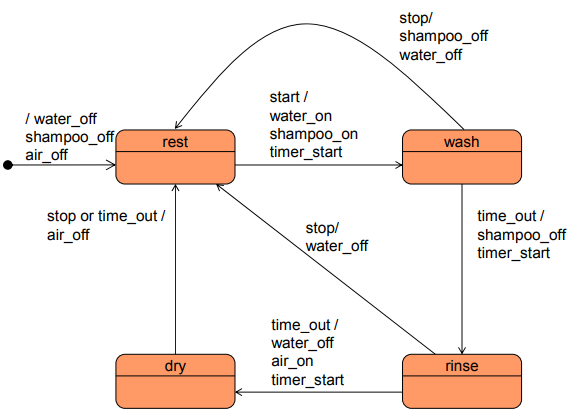
\includegraphics[width=\linewidth]{waschanlage_state_diagram.png}
    \begin{itemize}
        \item \textbf{rest}: Ausgangszustand
        \item \textbf{wash}: start / water\_on, shampoo\_on, timer\_start
        \item \textbf{rinse}: time\_out / shampoo\_off, timer\_start
        \item \textbf{dry}: time\_out / water\_off, air\_on, timer\_start
        \item Zurück zu rest: stop / water\_off, shampoo\_off, air\_off
    \end{itemize}
\end{example2}

\subsection{C-Implementation}

\begin{KR}{State Machine in C implementieren}\\
    \paragraph{Datenstrukturen}
    \begin{itemize}
        \item Enum für States: \texttt{typedef enum \{STATE1, STATE2\} state\_t;}
        \item Enum für Events: \texttt{typedef enum \{EVENT1, EVENT2\} event\_t;}
        \item Statische Variable: \texttt{static state\_t current\_state;}
    \end{itemize}
    
    \paragraph{Hauptschleife}
\begin{lstlisting}[style=basesmol]
int main(void) {
    event_t event;
    fsm_init();
    while (1) {
        event = get_event();
        if (event != NO_EVENT) {
            fsm_handle_event(event);
        }
    }
}
\end{lstlisting}
    
    \paragraph{FSM Handler (Switch-Case)}
\begin{lstlisting}[style=basesmol]
void fsm_handle_event(event_t event) {
    switch (current_state) {
        case STATE1:
            switch (event) {
                case EVENT1:
                    action1();
                    current_state = STATE2;
                    break;
                default:
                    // unbehandelte Events
                    break;
            }
            break;
        case STATE2:
            // ...
            break;
        default:
            current_state = INITIAL_STATE;
            break;
    }
}
\end{lstlisting}
    
    \paragraph{Event Detection}
    \begin{itemize}
        \item Polling: Regelmäßige Abfrage in Hauptschleife
        \item Interrupt-driven: Events in ISR in Queue einreihen
        \item Edge Detection: Flanken erkennen (static Variable)
    \end{itemize}
\end{KR}

\begin{example2}{LED-Steuerung State Machine}\\
    Spezifikation:
    \begin{itemize}
        \item WAIT: Beide LEDs aus, warten auf S0
        \item ALL\_ON: Beide LEDs an bei S0
        \item S0 oder S1 in ALL\_ON $\rightarrow$ entsprechende LED aus, zurück zu WAIT
    \end{itemize}
    
    \tcblower
    
    \textbf{Implementierung:}
\begin{lstlisting}[style=basesmol]
typedef enum {
    WAIT,
    ALL_ON
} fsm_state_t;

typedef enum {
    NO_SWITCH = 0x00,
    S0 = 0x01,
    S1 = 0x02
} event_t;

static fsm_state_t state = WAIT;

void fsm_handle_event(event_t event) {
    switch (state) {
        case WAIT:
            switch (event) {
                case S0:
                    led_turn_on(LED0_LED1);
                    state = ALL_ON;
                    break;
                default:
                    state = WAIT;
                    break;
            }
            break;
            
        case ALL_ON:
            switch (event) {
                case S0:
                    led_turn_off(LED0);
                    state = WAIT;
                    break;
                case S1:
                    led_turn_off(LED1);
                    state = WAIT;
                    break;
                default:
                    state = ALL_ON;
                    break;
            }
            break;
            
        default:
            state = WAIT;
            break;
    }
}
\end{lstlisting}
\end{example2}

\begin{remark}
    State Machines eignen sich besonders für reaktive Systeme mit klaren Zuständen und definierten Übergängen. Die Trennung von Event-Detection, State-Logic und Actions macht den Code wartbar und testbar.
\end{remark}